

\section{Experimental Setup}
\label{sec:airindia_15}
For the AE, the learning rate is $l_r = 10^{-4}$ with a reduction by a factor of $\Gamma = 0.1$ at every 2 training epochs. Optimization is performed using the ADAM solver with a momentum $\mu = 0.95$ and weight decay $\beta = 0.005$. The total labeled data is divided into 3 parts: training, test and validation which are selected at random. The proportions are 10\%, 30\% and 60\% of the total labeled data respectively. The training is balanced by selecting a fixed number of pixels per class randomly from the 10\% training pool. The accuracy statistics are reported as an average of 5 runs on the validation set. The FF network is trained in a supervised manner with $l_r = 10^{-5}$ , $\mu = 0.92$ and $\beta = 0.005$. The classification is obtained as output from the terminal layer of the FF network. 

% % CAN BE REMOVED FOR IGARSS
The training is proceeded under constraint of the cross-entropy error, which is monitored individually for the training and test datasets. If the cross-entropy error of the two datasets follow very nearly the same trajectory, it can be deduced that the network is under-fitting the dataset. On the contrary, if the trajectories are held at a constant, but significant offset, with the training leading the test, the network is over-fitting the data, leading to a better fit in the training samples, but poor performance in the test-set. In the ideal case, the training leads the curve of the test cross-entropy error with a moderate margin. The aforementioned hyper-parameters are tuned to achieve the same. 




\section{Results and Discussion}\label{Sec:ResultsDiscussion}
\label{sec:airindia_5}

\begin{figure}[htp]
\begin{subfigure}[b]{0.9\columnwidth}
\centering
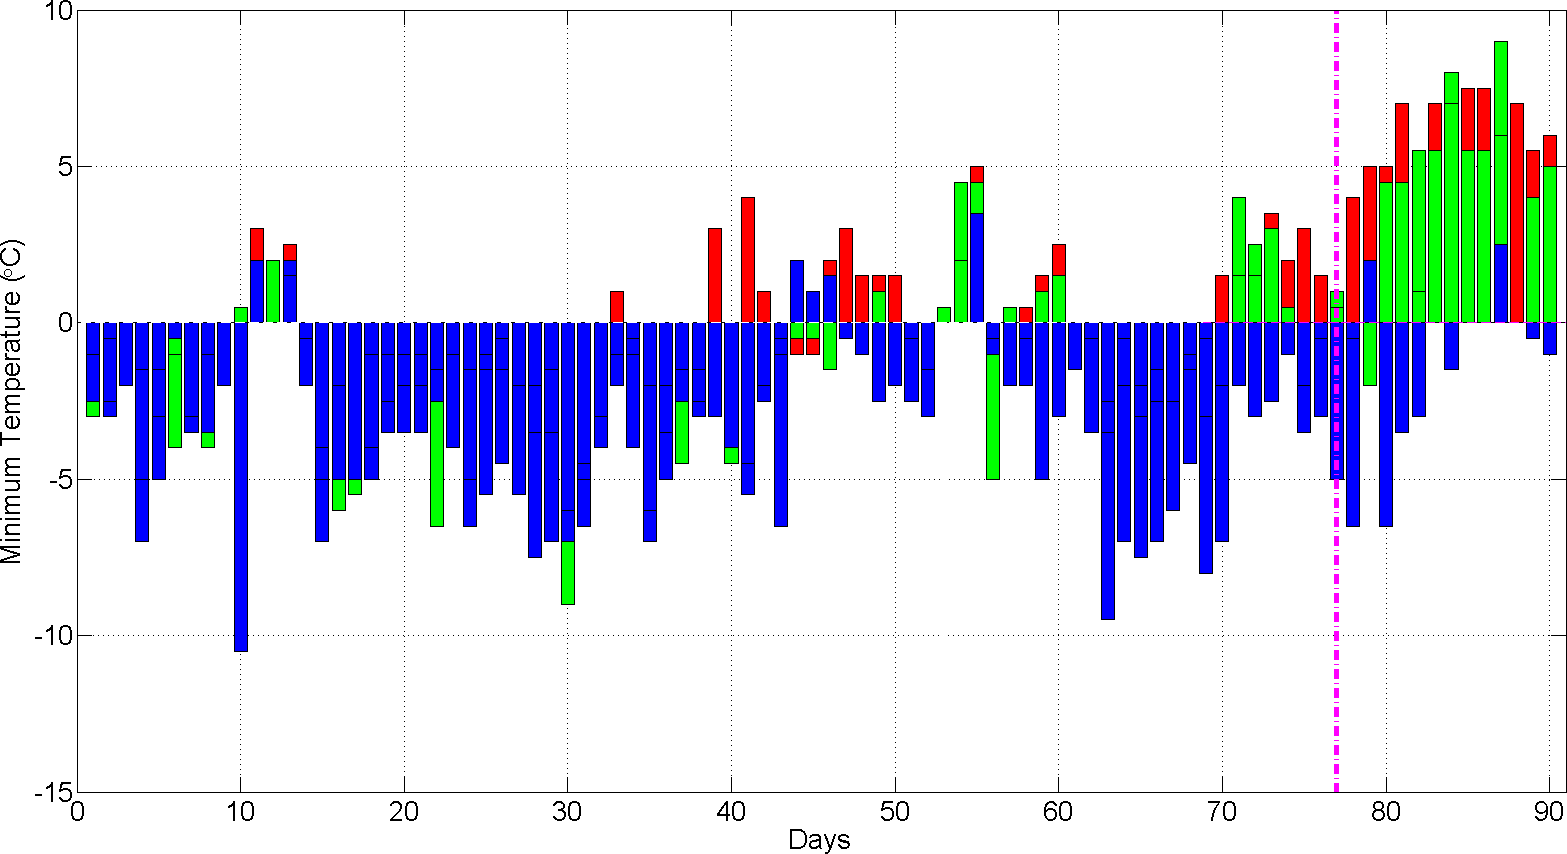
\includegraphics[width=0.7\columnwidth]{Figures/SnowCover2018/Oldfig/Minimum_Temperature_Vs_Days}
\caption{}
\end{subfigure}
~
\begin{subfigure}[b]{0.9\columnwidth}
\centering
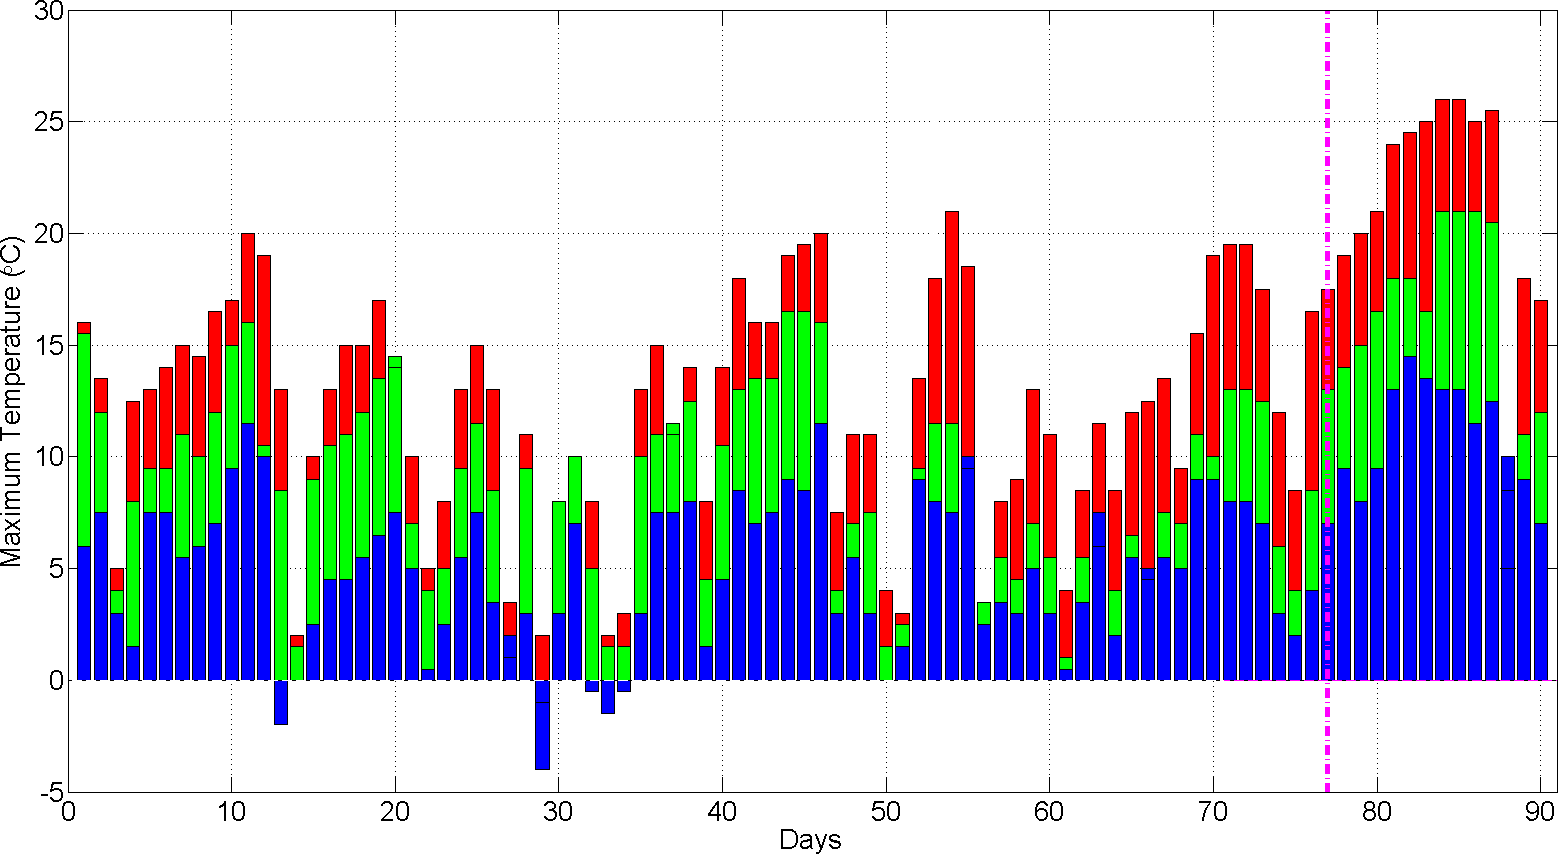
\includegraphics[width=0.7\columnwidth]{Figures/SnowCover2018/Oldfig/Maximum_Temperature_Vs_Days}
\caption{}
\end{subfigure}
\caption{Diurnal trends in (a) Minimum and (b) Maximum air temperatures from January to March 2015 with the dashed pink line denoting the day of the acquisition of the SAR scene (18th March, 2015). Data is courtesy the Bahang observatory.}
\label{fig:Diurnal}
\end{figure}

% % % %  Study area
In the lower altitude regions near the Bahang observatory, season wooded vegetative forests can be found to grow.
%
The altitude is low enough for the snow-cover to melt in the summer months, hydrating the under-soil and allowing support for vegetative growth. In the winter months, the forests usually lose their foliage, and precipitation leads to accumulation of snow in their branches. Diurnal fluctuations in temperature can lead to freezing as shown in Figure~\ref{fig:Diurnal}. 

In its frozen state, water is known to present a very different scattering signature than dry or wet snow, hence the forest structure even in the winter months, presents a very different scattering mechanism than the snow cover, allowing for discrimination. This is can be seen from the $H/\alpha$ analysis. 

This transformation can be accredited to drop in the moisture content of the trunk, branches, and twigs due to freezing weather conditions. Due to freezing, the dielectric constant of vegetation distinctively decreases. The conifer species demonstrates higher percentage increase in stiffness since its twigs which are more flexible under thawed conditions exhibits greater percentage increase in Young’s modulus when frozen~\cite{dobson1990effects}. Freezing causes an increase in the value of Young's modulus of twigs, branches, and trunks of trees. Sub-zero temperatures are known to increase the stiffness of woody plants. The stiffening of the wood at sub-zero temperatures increases due to the formation of ice crystals in cells of frozen wood which renders the branches more rigid. In the case of coniferous species, under warmer temperatures, the ice crystals within the cells liquefy which allows increased bending of branches to shed the intercepted snow. The thin film of dry snow, if present, on the branches will be transparent at C-band~\cite{bernier1998potential}.

Two common classes over the region were considered for all the analysis, viz. bare ground over which negligible or extremely sparse vegetation is present, and the forested area. A seasonal variation in the $H/\alpha$ parameters are conducted in this study over the bare snow-covered ground and the forested
areas. The seasonal response of the terrain in the $H/\alpha$ plane corresponding to specific scattering characteristics (or zones) with multi-temporal images is shown in Figure~\ref{fig:halpha_scat}. The figure shows the possible combination of $H$ and $\alpha$ to form specific classes based on the properties of scattering mechanisms.

During February and March, the study area witnessed a substantial amount of precipitation in the form of snowfall. The areas which were bare during rest of the year were covered with snow during winters. An increase in the value of both $\alpha$ and $H$ was observed over the bare-ground.
%
Also, the polarimetric signatures for a forest patch and a bare ground covered by snow are plotted in Figure~\ref{fig:signatureanal} . As can be seen, the scattering mechanisms for the two classes are very different. 

\begin{figure}
\centering
\begin{subfigure}[t]{0.35\columnwidth}
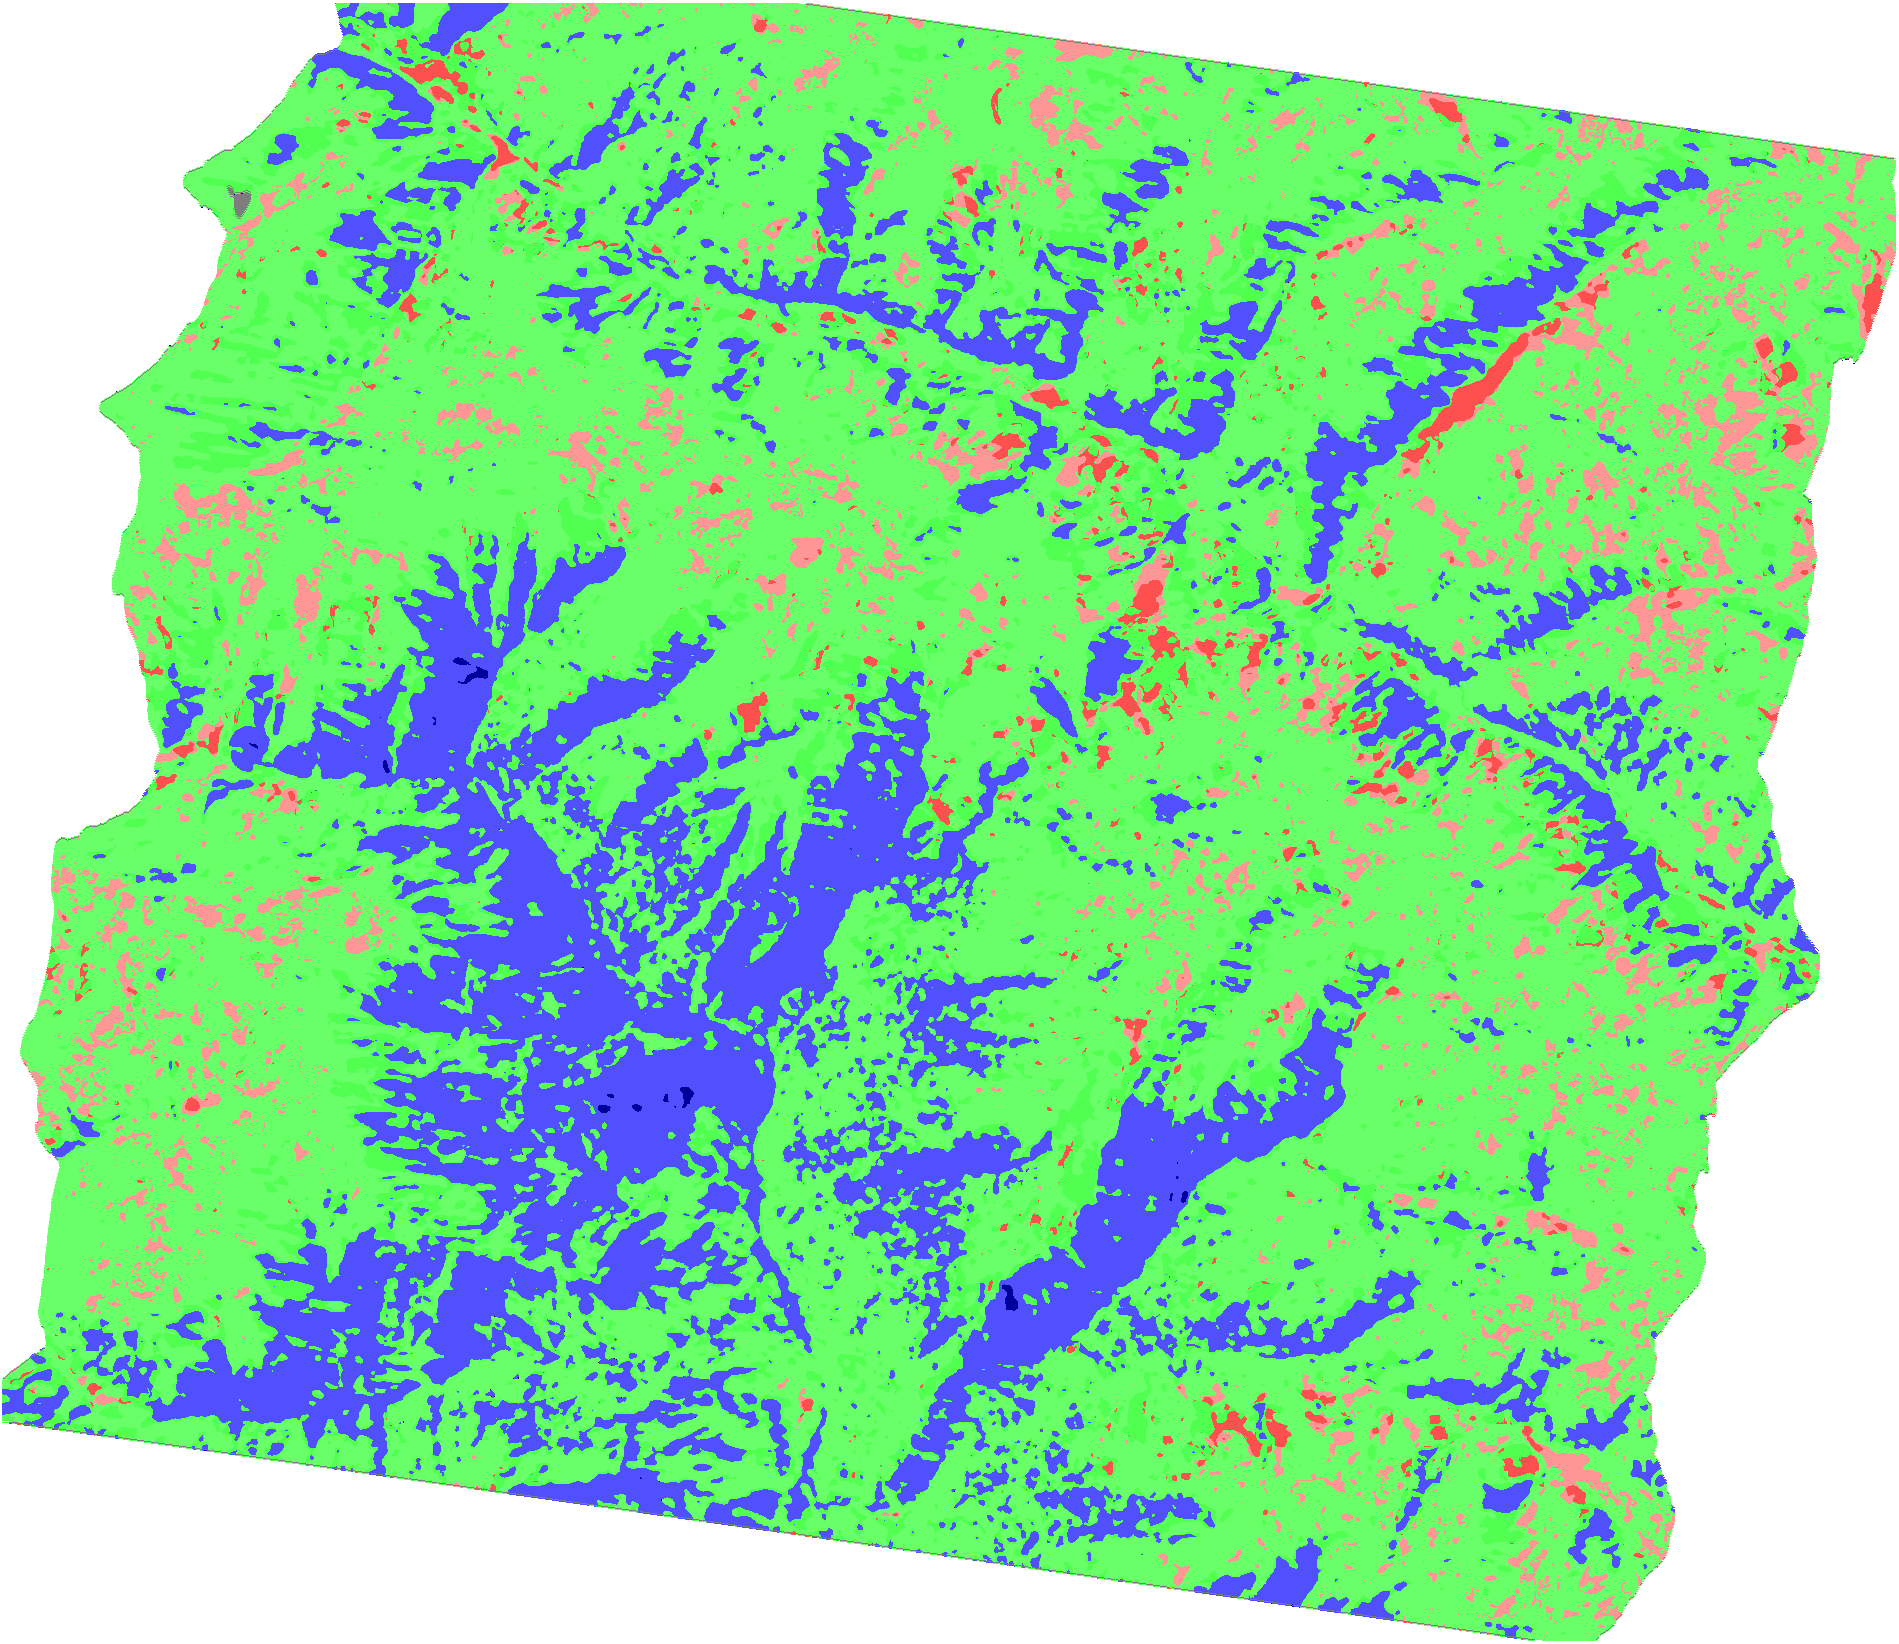
\includegraphics[width=\columnwidth]{Figures/SnowCover2018/Oldfig/H_alpha_class_mar_2015}
\caption{}
\end{subfigure}
~
\begin{subfigure}[t]{0.3\columnwidth}
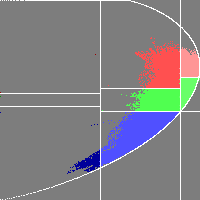
\includegraphics[width=\columnwidth]{Figures/SnowCover2018/Oldfig/H_alpha_segmented_plane_mar_2015}
\caption{}
\end{subfigure}
\caption{(a) $H/\alpha$ class map along with (b) $H/\alpha$ segmented plane for the March 2015 acquisition.}
\label{fig:halpha_scat}
\end{figure}


\begin{figure}
\centering
\begin{subfigure}[t]{0.45\columnwidth}
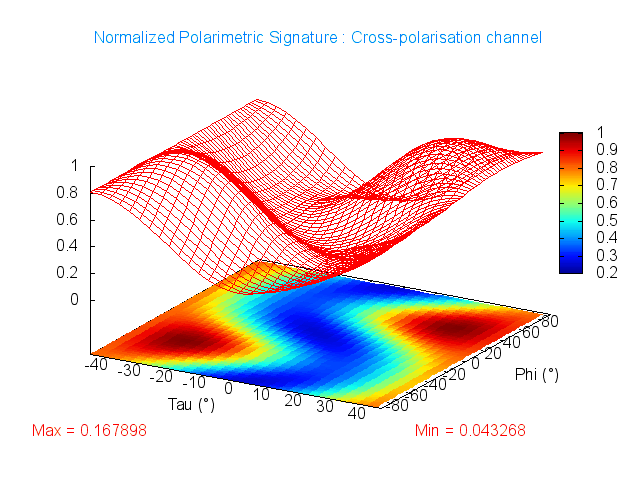
\includegraphics[width=\columnwidth]{Figures/SnowCover2018/Sig/CopolSignature_1085_492_Snow}
\caption{}
\end{subfigure}
~
\begin{subfigure}[t]{0.45\columnwidth}
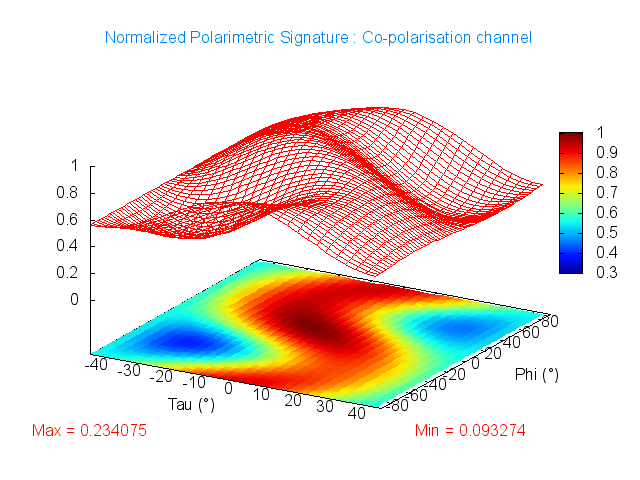
\includegraphics[width=\columnwidth]{Figures/SnowCover2018/Sig/XpolSignature_1085_492_Snow}
\caption{}
\end{subfigure}
~
\begin{subfigure}[t]{0.45\columnwidth}
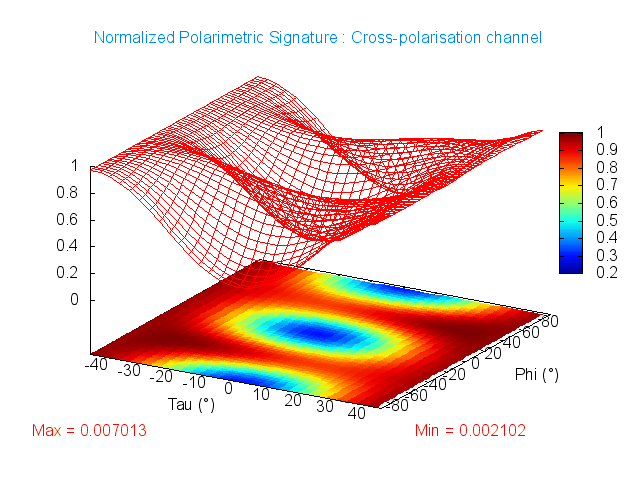
\includegraphics[width=\columnwidth]{Figures/SnowCover2018/Sig/CopolSignature_forest_675_1125}
\caption{}
\end{subfigure}
~
\begin{subfigure}[t]{0.45\columnwidth}
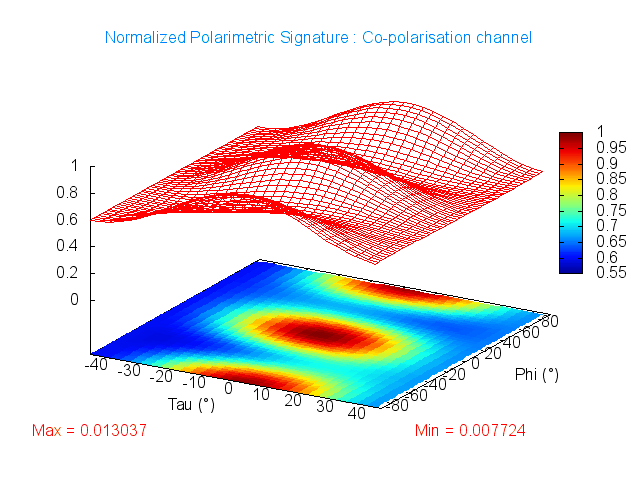
\includegraphics[width=\columnwidth]{Figures/SnowCover2018/Sig/XpolSignature_forest_675_1125}
\caption{}
\end{subfigure}
\caption{Linear Scale plots of (a) Co-pol and (b) Cross-pol polarimetric signatures over snow covered bare ground and (c) Co-pol and (d) Cross-pol polarimetric signatures over forested areas.}
\label{fig:signatureanal}
\end{figure}



% % % AUTOENCODER

%% 1. Compare reconstruction accuracy -RnD 
The original and re-constructed $M_{11}$ element is presented in Fig.~\ref{fig:ae_re}. As seen, the reconstruction $X'$ closely follows the original input $X$, but, with a non-liner transformation. This transformation and happens independently on each dimension of the input. This leads to the generation of a representational feature manifold, which has improved separability for classification over the original input space.
%
%2. Talk about features
For visualization and understanding the action of the AE, two input space features are selected and presented in a scatter plot, along with two features from the representational space in Figure~\ref{fig:AE_M_comp}. The feature combinations are selected at random.
%3. Show feature thumbnails


\begin{figure}
\centering
\begin{subfigure}[b]{0.45\textwidth}
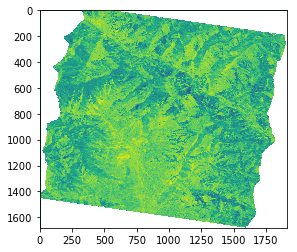
\includegraphics[width=\textwidth]{Figures/SnowCover2018/0_og}~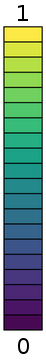
\includegraphics[height=3cm]{Figures/SnowCover2018/scale} 
\caption{}
\end{subfigure}
~\quad
\begin{subfigure}[b]{0.45\textwidth}
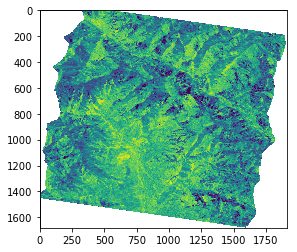
\includegraphics[width=\textwidth]{Figures/SnowCover2018/0}~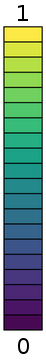
\includegraphics[height=3cm]{Figures/SnowCover2018/scale}
\caption{}
\end{subfigure}
\caption{A comparison of the (a) original and (b) reconstructed $M_{11}$ element from the AE shown normalized between 0 to 1. }
\label{fig:ae_re}
\end{figure}

\begin{figure}
\centering
\begin{subfigure}[b]{0.45\textwidth}
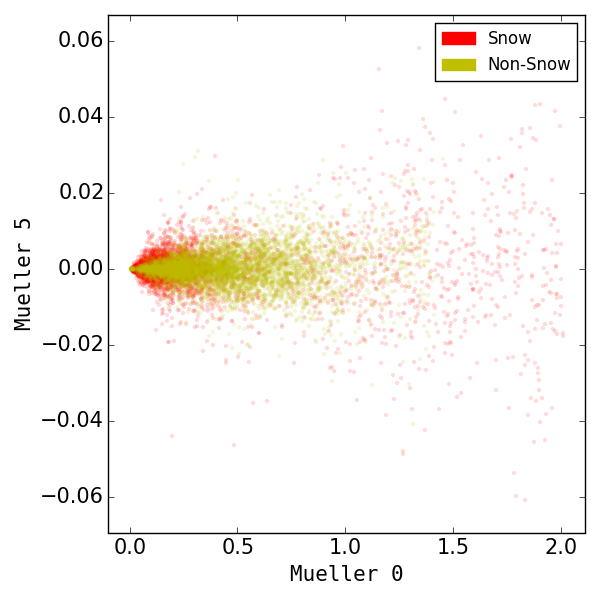
\includegraphics[width=\textwidth]{Figures/SnowCover2018/Mueller/0_5}
\caption{}
\end{subfigure}
~
\begin{subfigure}[b]{0.45\textwidth}
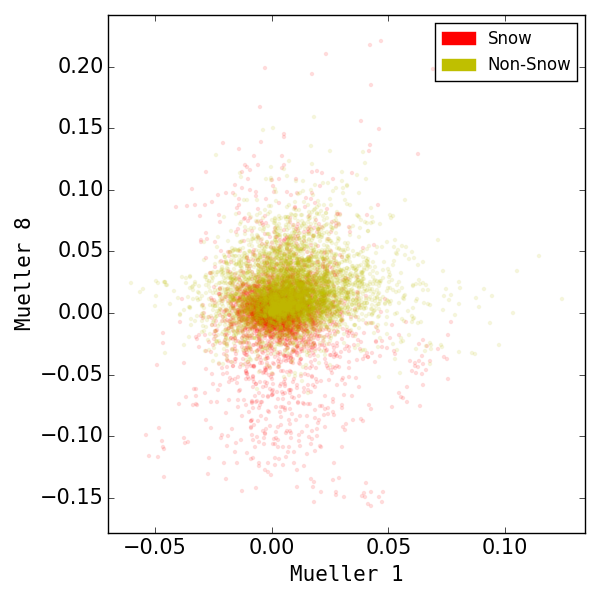
\includegraphics[width=\textwidth]{Figures/SnowCover2018/Mueller/1_8}
\caption{}
\end{subfigure}
~
\centering
\begin{subfigure}[b]{0.45\textwidth}
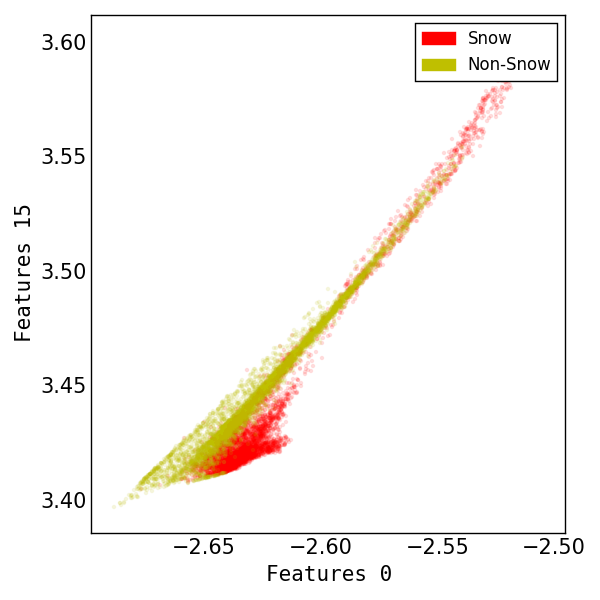
\includegraphics[width=\textwidth]{Figures/SnowCover2018/AE/0_15}
\caption{}
\end{subfigure}
~
\begin{subfigure}[b]{0.45\textwidth}
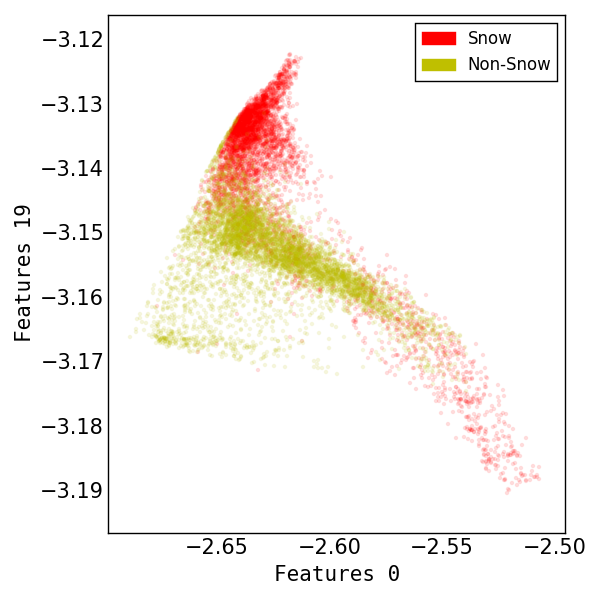
\includegraphics[width=\textwidth]{Figures/SnowCover2018/AE/0_19}
\caption{}
\end{subfigure}
\caption{A comparison of some (a,b) Mueller (c,d) AE Representation layer features extracted from the full polarimetric image. }
\label{fig:AE_M_comp}
\end{figure}




% Snow-Cover Discussion
It can be seen in Figure~\ref{fig:results} that snow is undetected in the forested zone located towards the lower elevations of the area. The results correlate well with the snow-cover maps derived from the optical Landsat-8 data by the NDSI technique. Due to the inherent imaging differences between radar and optical sensors there is disparity in the observed percentage snow-covered/snow-free areas. 
%
The algorithm is able to segregate the snow-covered high elevation areas from the snow-free canopies. Due to differences in the scattering mechanisms over the frozen forest and porous snowpack, the representations captured by the AE were different for both these classes. Distinct class representations enabled the network to perform well in the final classification stage. 

\begin{figure}
\centering
\begin{subfigure}[b]{0.45\columnwidth}
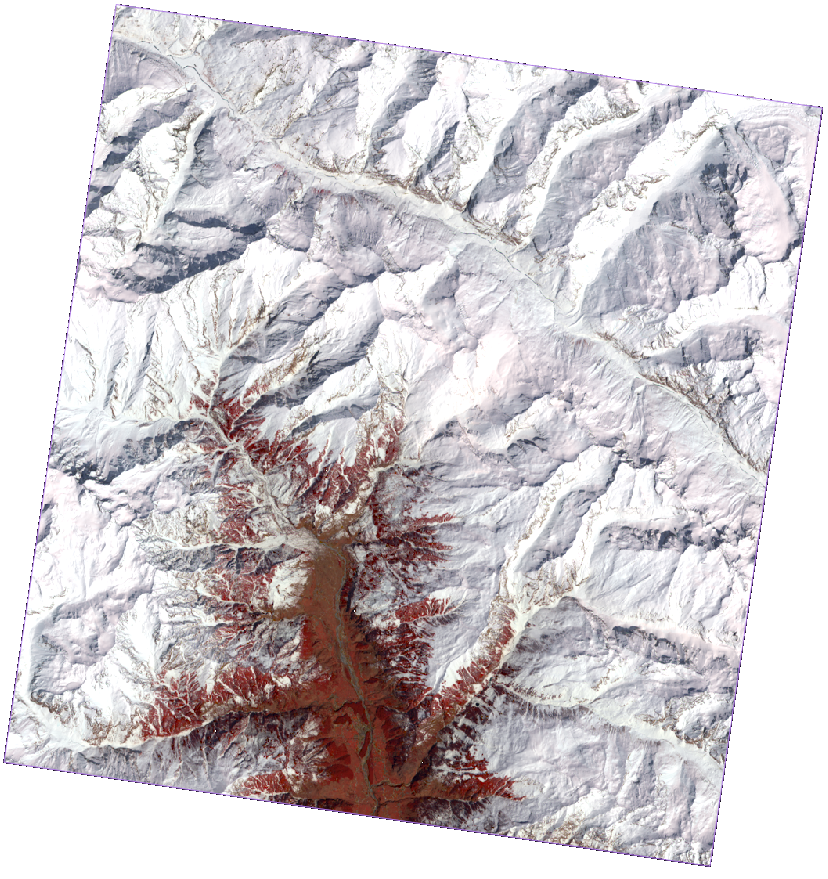
\includegraphics[width=\textwidth]{Figures/SnowCover2018/FCC}
\caption{}
\end{subfigure}
~
\begin{subfigure}[b]{0.45\columnwidth}
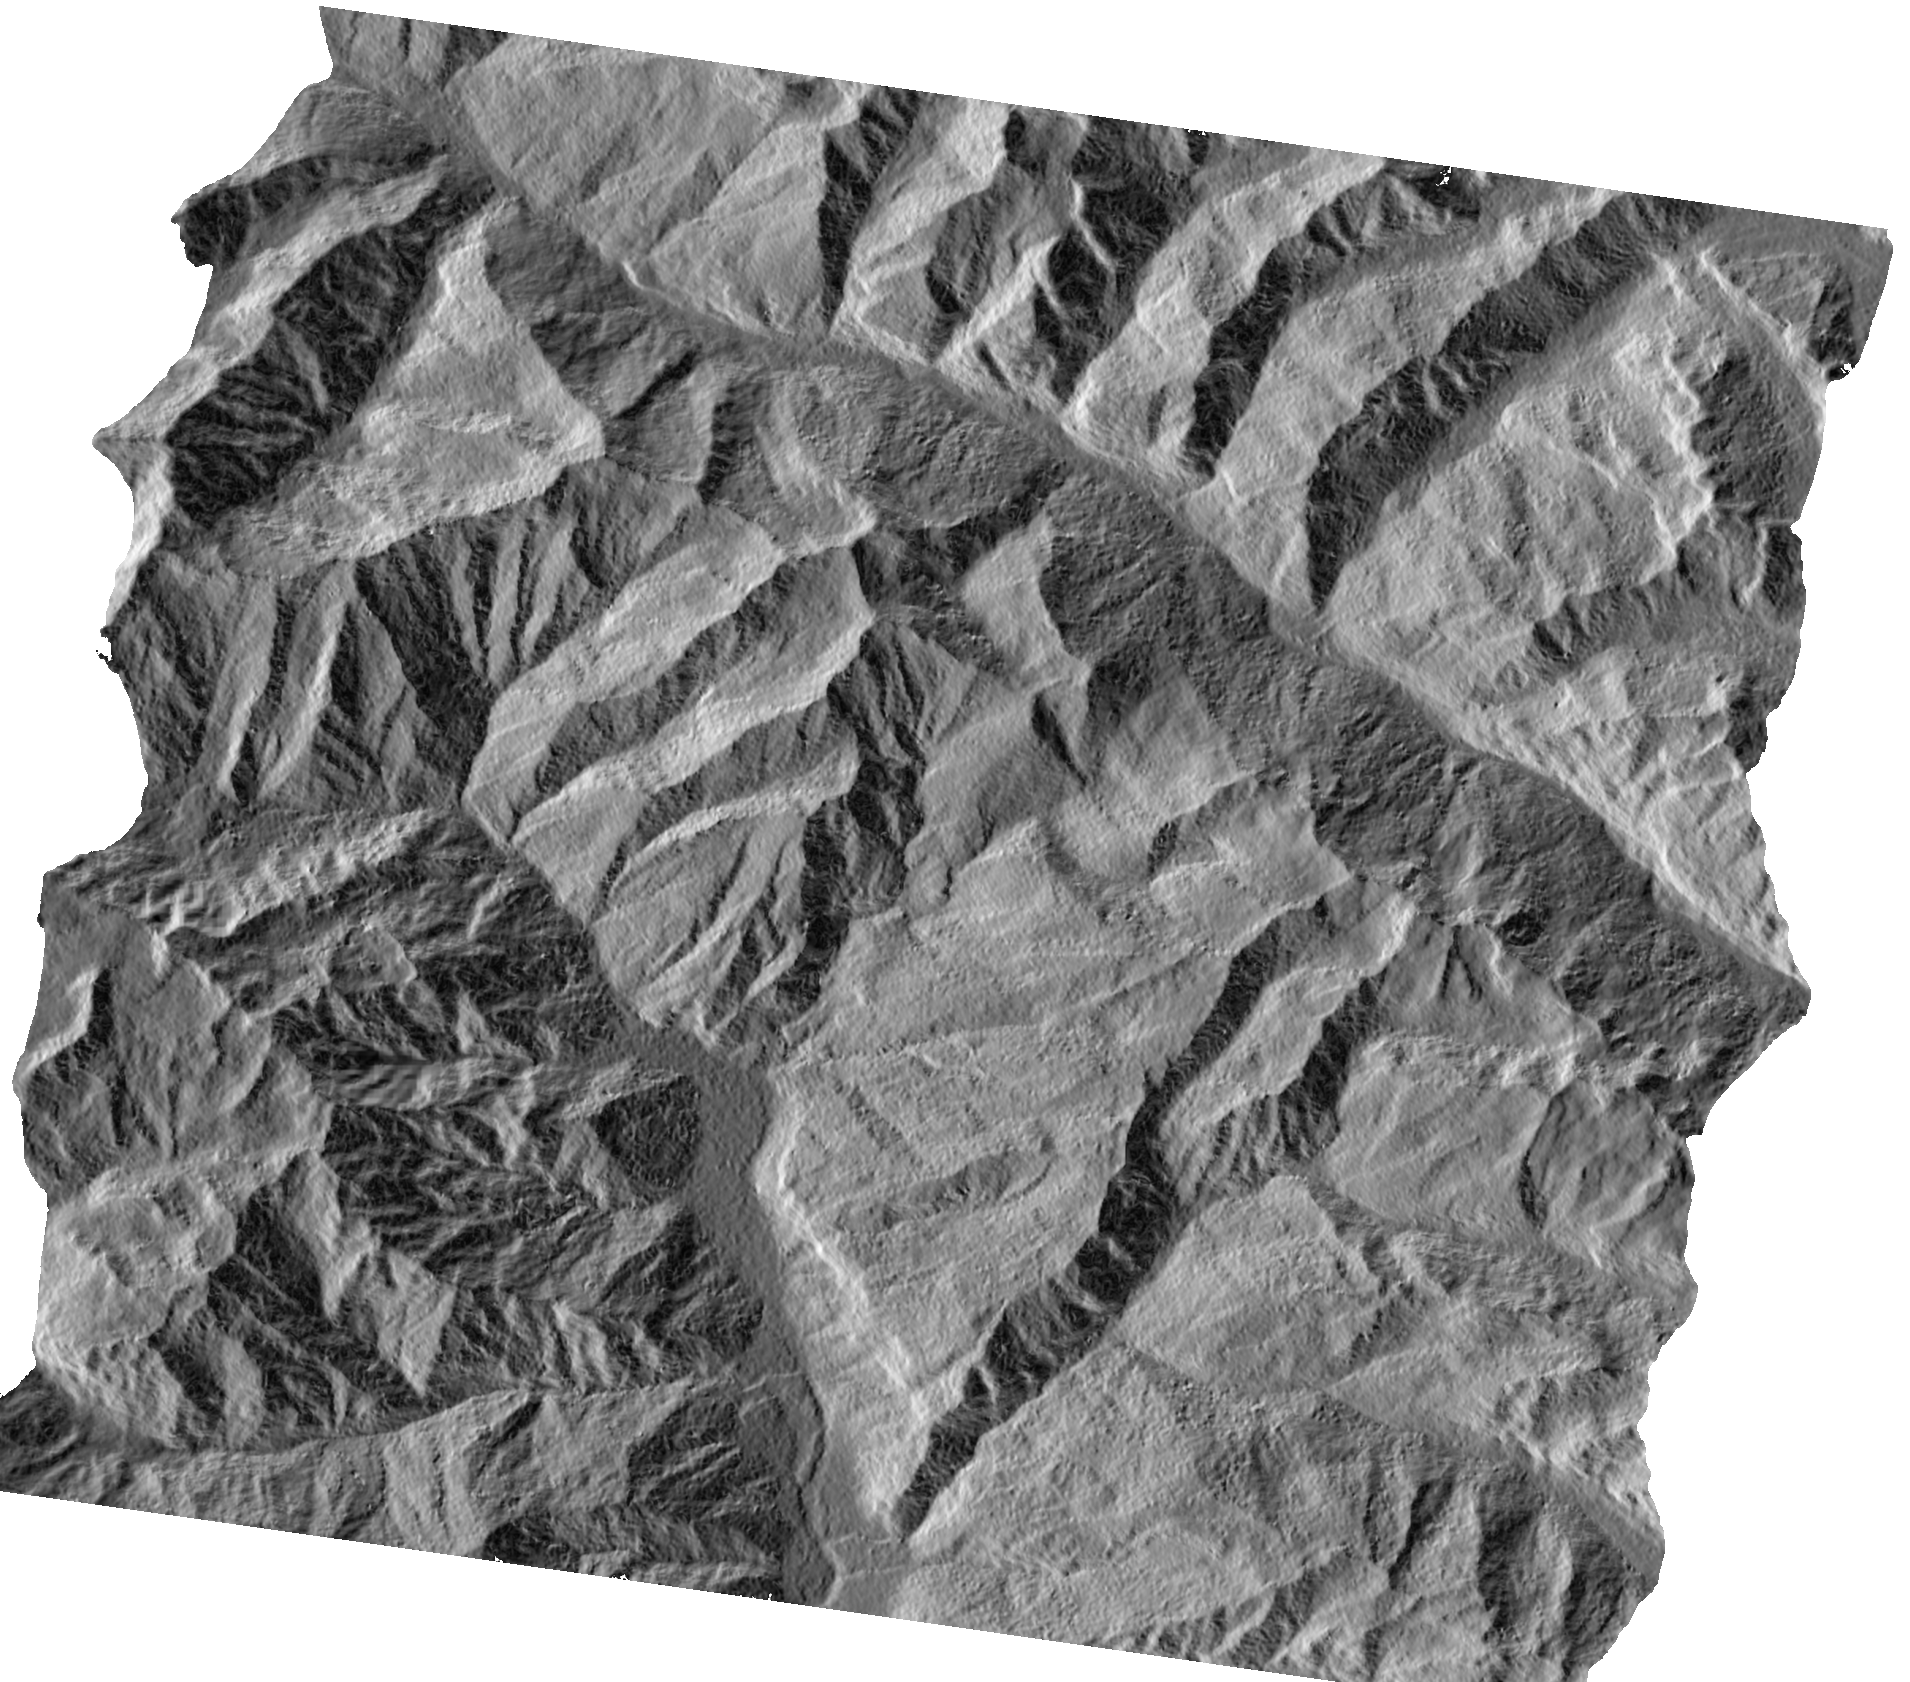
\includegraphics[width=\textwidth]{Figures/SnowCover2018/IncAng2}
\caption{}
\end{subfigure}
~
\begin{subfigure}[b]{0.45\columnwidth}
\includegraphics[width=\textwidth]{Figures/SnowCover2018/Hyb}
\caption{}
\end{subfigure}
~
\begin{subfigure}[b]{0.45\columnwidth}
\includegraphics[width=\textwidth]{Figures/SnowCover2018/Lin} 
\caption{}
\end{subfigure}
\begin{tabular}{cccc}

\includegraphics[width=0.04\columnwidth]{Figures/SnowCover2018/Snow} & Snow & 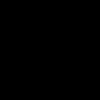
\includegraphics[width=0.04\columnwidth]{Figures/SnowCover2018/NoSnow} & No-Snow/Shadow
\end{tabular}
\vspace{3em}
\caption{(a) False color composite of the area collected by Landsat-8 and the (b) DSM of the area. Resultant snow maps using (c) hybrid polarimetric and (d) full polarimetric data.}
\label{fig:results}
\end{figure}

The primary difference in the snow-cover map obtained from the optical and radar images occurred as a result of layover/shadow effects and selective penetration in radar images. Selective penetration can modify the scattering signatures which can consequently result in training with erroneous representation and thus a misclassification. The images were also acquired on different dates which contributes towards the mismatch.          

% % % % % % % % % % % % % % % % % % % % % % % % % % % % % % % % % % % % % % % % % % % %
% Compact Pol VS Full Pol
The difference in the two snow cover maps obtained from the combination of linear polarization and that of the circular polarization are more evident over the forest areas. This can be attributed to the difference in the received scattering mechanism observed at the sensor for the two different incident waves. This could be predominantly because of the scattering types prevailing over the respective areas. 

% Polarization Signatures

However in the snow laden bare fields, the two different polarizations show similar results. It would be interesting to find an optimized incident polarization that might optimize performance in snow-cover mapping. 




% \begin{figure}
%     \centering
%     \begin{subfigure}[b]{0.3\textwidth}
%         \centering
%         \includegraphics[width=\textwidth]{Figure/Hyb}
%         \caption{}
%         \label{fig:hyb}
%     \end{subfigure}
%     \hfill
%     \begin{subfigure}[b]{0.3\textwidth}
%         \centering
%         \includegraphics[width=\textwidth]{Figure/Lin}
%         \caption{}
%         \label{fig:lin}
%     \end{subfigure}
%     \caption{Resultant snow maps using (a) Hybrid and (b) Full Pol data}
%     \label{fig:result}
% \end{figure}





